\chapter{Introduction to the CoreASIM Language, Interpreter, and ICEF}
\label{ch:CoreAsimIntro}

\vspace{-1cm}
\begin{center}
Eduard Hirsch
\end{center}

In this chapter an overview of the used technologies for running the INTERLACE Specification is given. At the beginning a quick start description is provided in order to jump right into the execution of the model.

Further details which are enabling the Abstract State Interacting Machines (ASIM) specifications to be executed are discussed and why this possible in a simple and stable manner.

\section{Quick Start Vagrant}
\label{sec:quick-start-vagrant}

There are two base environments available. One based one docker and one based on vagrant. The focus shifted from the vagrant environment which can be downloaded at github\footnote{https://github.com/InterlaceProject/ASIMVagrantEnvironment} to a docker based version which is explained in section \ref{sec:quick-start-docker}. Nevertheless, for developer preferring vagrant, the setup will be still explained.

The vagrant definition provides a running environment for executing the INTERLACE ASIM definitions. During the provisioning process an ubuntu vagrant box is set up which installs the necessary components on that box. It is cloning and building the ICEF framework\footnote{https://github.com/biomics/icef} as well as the ASIM Specification\footnote{https://github.com/InterlaceProject/ASIMSpec} into the data directory where it is finally ready for usage.

\subsection{Prerequisites}

Download and install the following software products:

\begin{itemize}
	\item Virtual Box: https://www.virtualbox.org/
	\item git: https://git-scm.com/downloads
	\item vagrant: https://www.vagrantup.com/
\end{itemize}

\subsection{Clone Environment}

To clone the ASIM vagrant environment from github into a directory git can be utilized:

\begin{lstlisting}
	git clone https://github.com/InterlaceProject/ASIMVagrantEnvironment.git
\end{lstlisting}

\subsection{Execution}

Once all software components are installed and the vagrant definitions are cloned it is possible to call

\begin{lstlisting}
	execute.sh
\end{lstlisting}

from the main directory in order to let the INTERLACE specifications run. Note: when using Windows it is necessary to start that command within git-bash which needs to run in elevated admin mode (right click $\rightarrow$ start as administrator).

On the very first execution the script is provisioning a virtual machine based on ubuntu by calling \texttt{vagrant up} which may take some time. Consecutive calls will be much faster. A detailed description explaining the precise process is covered in section \ref{sec:exec-env-model-details}.

Once the execution is started it will run until it is stopped by pressing \textbf{ctrl + c} or by calling

\begin{lstlisting}
	stop.sh
\end{lstlisting}

from any other console window.

\section{Quick Start Docker}
\label{sec:quick-start-docker}

The docker project at github\footnote{https://github.com/InterlaceProject/ASIMDockerEnvironment} is also based on virtualization like the vagrant environment but emphasizing \textit{Operating System} instead of \textit{Hardware virtualization}\footnote{https://www.docker.com/what-container\#comparing}.

\subsection{Prerequisites}

\begin{itemize}
	\item install docker
	\item install git (including git bash for windows)
\end{itemize}

On Linux machines it is important to add the current user to the docker group in order to manage docker container and images. Otherwise all further explained commands need to be executed as root or with sudo.

For Windows machines use \textit{git-bash} to execute the commands described in the following sections.

\subsection{Before First Execution}

In order to configure the environment it is necessary to call the following script:

\begin{lstlisting}
	./configure
\end{lstlisting}

This will generate a docker container image called \textit{asim} where all the necessary frameworks are build and prepared for execution of the specifications. The ICEF framework as well as the ASIM model specifications are cloned outside of the container to simplify development.

\subsection{Execute Specification}

The container image \textit{asim} created during the configuring step can be started by calling

\begin{lstlisting}
	./execute
\end{lstlisting}

A container started in this way is called \textit{active\_asim} and running all the necessary steps like starting an ICEF manager as well a ICEF brapper to run the ASIM specifications.

Like the vagrant environment a running execution may be stopped by pressing \textbf{ctrl + c}.

\section{Execution Environment Stack}
\label{sec:exec-env-stack}

Independent of the used virtualization techniques a consistent base system is used. So both docker as well as vagrant are provisioning a Linux based operating system using an Ubuntu 16.04 LTS (Long Term Support) distribution.
That consistent, stable and reliable structure will be important later when considerations about provability as well testability come into place. That design provides always the same preconditions and everybody executing or testing against the specifications will receive the same results.

\subsection{Software Stack}
\label{sec:env-exec-stack-software-stack}

The Ubuntu 16.04 LTS distribution is enhanced and updated according to the needs of an ASIM executing machine as well as to the needs of developers working with that virtual system. To be more specific the following components are installed during the provisioning process:

\begin{itemize}
	\item curl $\rightarrow$ Tool for querying REST resources (used for downloading package resources)
	\item nodejs $\rightarrow$ JavaScript engine including the package manager npm (running the Manager Component of ICEF)
	\item build-essential $\rightarrow$ Packages needed to compile a debian based package (used for building the project sources)
	\item maven $\rightarrow$ Java build and packaging tool (used for building the project sources)
	\item vim $\rightarrow$ Well known U/Linux editor (for development purposes)
	\item git $\rightarrow$ Distributed Version Control System (downloading source repositories from GitHub)
	\item Java 8 $\rightarrow$ Programming Language used for coreASIM base system implementation (running ASIM instances)
\end{itemize}

\subsection{Provisioning Process}

The provisioning process can be separated into 3 steps which are executed when \textit{.\/configure} for docker or \textit{vagrant up} for vagrant is called from the command line:

\begin{enumerate}
	\item Download ASIMSpec and ICEF from GitHub
	\item Install of software packages mentioned in section \ref{sec:env-exec-stack-software-stack}
	\item Build ICEF framework and prepare virtual machine for execution
\end{enumerate}

For development purposes the ASIMSpec as well as the ICEF framework are cloned into directories which are available from the host machine and the virtual guest machine. This is necessary because then it is possible to directly edit the source or debug from outside and execute the code from within the container. Consequently it is not necessary to copy the code into the container when changes where done.

For \textbf{Vagrant} a shared folder is configured over the vagrant file shown here

\begin{lstlisting}
	...
	config.vm.synced_folder "./data", "/vagrant-data"
	...
\end{lstlisting}

is referring to the fact that on the host system the folder \textit{data} is used and on the guest system a folder \textit{vagrant-data} is mounted. Those folder are shared and thus containing the same content. Additionally during provisioning a symbolic link in the home directory is created called project (\textit{/home/ubuntu/project}) which is linking the mounted root folder /vagrant-data.

When the virtual machine is stopped the data directory on the host is kept and can be still manipulated or executed (of course only if the framework dependencies are installed on the host as well).

For \textbf{Docker} we need to first clone all GitHub sources to the host machine and can only then share the files into the guest container by using the command line option "-v"

\begin{lstlisting}[language=bash]
	docker run -v "$1/ASIMSpec:/home/ASIMSpec" \
	           -v "$1/icef:/home/icef" \
	           --name active_asim -it asim /$2
\end{lstlisting}

This line is part of the script \textit{scripts/runDocker.sh}. \$1 here stands for the local directory of the environment and \$2 is normally defaulted to the main execution script started inside the docker container. Important to note is that the \textit{ASIMSpec} folder of the host machine is shared into \textit{/home/ASIMSpec} of the docker container and the \textit{icef} directory is shared into \textit{/home/icef}.

\subsection{Execution}
\label{sec:env-exec-stack-exe}

The execution stack in figure \ref{fig:icef-intro-asim} shows where a ICEF specification is transmitted to for it to be executed. The details will be covered in section \ref{sec:icef-intro}. In this part of the document, however, we will take a look at how and which services are started.

Due to limitations of the ICEF framework it is currently not possible to cleanly shut down a running ICEF simulation with several running ASIM instances. Therefore both environments have to start and stop all services for every execution in order to grant a correct execution set-up.

\subsubsection{Start Services Processes}: Both environments offer a script (\textit{execute(.sh)}) to be called from the host system and one from within the virtualized machine (\textit{executeASIMSpec.sh/executeOnGuest.sh}). Whereas the script on the virtualized system only differ in directory references the outside scripts are need to handle different things as one script is dealing with docker and the other with vagrant.

In detail Docker can immediately start the servers and run the script inside the container whereas vagrant needs add an additional step if the virtual machine is not up and running yet. Thus vagrant

\begin{enumerate}
	\item is trying to start the server processes and submit the specifications
	\item if the first step failed is checking for the virtual machine if it is running and if not it tries to restart the virtual machine
	\item if the restart has been successful the first step will be retried.
\end{enumerate}

When now focusing on the first step which is basically the same on both environments it can be discussed in detail how the process is continued. So on the guest system we are first running a so called \textit{CASIMA} which is short hand for coreASIM-Manager \ref{sec:icef-intro}. This manager takes care about ASIM states, scheduling and also acts as messaging backbone.

Next a second service process is started. The service is a wrapper for the coreASM implementation and its name is Brapper (BIOMICS wrapper). This Brapper service executes enhanced ASM code named BSL that offers additional language primitives specifically designed during the BIOMICS project. Those features mainly include interaction features used to model biochemical systems, nevertheless, and actually because of that they are also suitable for decentralized and distributed computer system.

When a Brapper is going to be started it needs to be register at a manager instance. As described in section \ref{sec:icef-intro} it is possible to start multiple Brappers. Once a simulation is submitted to the manager, the manager is distributing the different simulations including their ASIMs to different Brapper services for executing them there trying to spread the load equally.

For the sake of simplicity the environment starts only one Brapper by default. In the final implementation it'll be possible to configure the number of Brappers used for execution.

\subsubsection{Submit ICEF definition file}: Finally after the service processes are running it is possible to submit a specification file to the manager. This is done by the executing bash script which is calling a  nodejs client:

\begin{lstlisting}
	...
	node loadICEF.js $project/ASIMSpec/run.icef localhost 9090
	...
\end{lstlisting}

The above listing uses a \textit{\$project} variable containing the path of ASIMSpec to find the icef specification. By convention the icef definition file of the ASIM Specifications is called \textit{run.icef} to clearly identify the entry point for the environment.
The last two parameters for the script are host as well as port where the manager services is running and waiting for requests.

\subsection{Development}
\label{sec:development}

For developing new simulations it is important to have a proper development environment. There are existing many IDE/Tool/Debuggers for Java and JavaScript which are used for Brapper, Manager or coreAS(I)M plugin development but there are only limited IDE choices for implementing AS(I)Ms.

For the public Integrated Development Environment Eclipse, developers of the ICEF framework have adopted the coreASM plugin for supporting the additional language primitives. Thus for working with ASIM implementations of INTERLACE you ideally DO NOT download the coreASM package which is available at the market place of Eclipse. The adopted plugin working with the new language elements is provided by the ICEF framework but is needed to build and imported manually into Eclipse.


\textbf{Import/Install of the IDE Eclipse plugin for coreASIM}
\begin{description}
	\item[Build Framework] For adding the ASIM plugin to Eclipse it is required to build and install the coreASIM plugin manually first because it is not downloadable from the Eclipse marketplace and only available as source version delivered with the ICEF framework and part of the coreASIM engine. Building and installing can be done by calling
	\begin{lstlisting}
		cd icef/coreASIM/org.coreasim.parent && mvn package install
		cd icef/coreASIM/org.coreasim.eclipse && mvn package install
	\end{lstlisting}
	Note that the icef directory is placed on different folders in the two environments!
	
	\item[Install Plug-In Development Environment in Eclipse] To install the ASIM Plug-in it is necessary to first add another Plug-in called Eclipse PDE (Plug-In Development Environment) from the marketplace for the current Eclipse installation or get a distribution which already contains that Plug-in.
	
	\item[Import Plugin as Project] Next the plugin needs to be imported to the workspace which can be done in Eclipse using the import wizard. To reach the wizard go to "File" $\rightarrow$ "Import...", search for "Existing Projects into Workspace" and click to get to "Import Project"-Window. Then click "Finish" to import the project.
	
	\item[Dry-Run Eclipse with coreASIM-Plug-In] This optional step can be done to check if the Plug-In is working correctly. For that it is necessary to right click the imported eclipse project and go to "Run As" $\rightarrow$ "Eclipse Application". Then a second Eclipse instance is started but this time a new tab should appear named "coreASIM" as well as when opening a file with extension \textit{casim} the ASIM definition should be syntax highlighted.

	\item[Enable the Plug-In] If the (optional) dry-run has been successful the export wizard will export the Plug-In into the running Eclipse installation by opening "File" $\rightarrow$  "Export" then choosing "Deployable Plug-ins and fragments" in the new Dialogue. The window which is opened next will offer to export fragment  \textit{org.coreasim.eclipse} by selecting the check box beside. Before clicking finish the combo box "Install into host" has to be chosen.
	
\end{description}

When finishing these steps on restart Eclipse offers a new tab in the top menu bar called "CoreASIM".

\textbf{Note on the installation}: When using the \textit{docker}-Environment you could skip the first step \textbf{Build Framework}, because all the necessary build steps are covered by the initial configuration script. Also a separate installation of the Eclipse Plug-In Development Environment (PDE) might omitted because it usually comes in a bundle with most standard J2EE installations of Eclipse.

\textbf{Notes on the Docker environment}
\label{sec_inner:note-docker}

Normally the ASIM Specifications are started by calling \textit{execute} from the main directory which is starting a script which will run the services and sent the ICEF definition. When stopping the container it instantly goes back to his original state before execution. Only the shared directories ASIMSpec and icef keep changes.

If it is necessary or convenient, like if the host is missing development packages (e.g. maven, nodejs, ...) which are available inside the container, it is possible to work from within the container by calling

\begin{lstlisting}
	./execute /bin/bash
\end{lstlisting}

which starts the docker container, runs a bash shell, keeping the STDIN open and connect a pseudo TTY. In this way it is possible to work with that bash shell, similar to connecting to a machine over SSH.

\section{ICEF - The Interaction Computing Execution Framework}
\label{sec:icef-intro}

The interaction framework is wrapping the original coreASM framework in order to extend it and giving it the capabilities to execute concurrent and distributed. It has been developed in a project called BIOMICS and financed by the European Commission.

\textbf{This wrapping took place on three levels:}

\textbf{First} the interpreter coreASM had to be extended supporting additional languages primitives as well as communications features. Here BSL replaces ASM as a new language having a new interpreter coreASIM.

\textbf{Second} a place has been created were the now so called Abstract State Interaction Machines (ASIMs) take over and are able to execute in parallel. This environment is called Brapper (short for BIOMICS Wrapper).

\textbf{Third} a central server called manager takes care handling distributed Brapper instances dealing with message and scheduling issues.

Technology wise coreASIM changes the coreASM implementation in Java. Brappers are written in Java as well but the managers are coordinating the Brappers using nodejs and therefor written in JavaScript.

\subsection{Framework Stack}

Next, the framework stack of ICEF in terms of the INTERLACE implementation is described more detailed. In figure \ref{fig:icef-intro-asim} the stack can be viewed in different levels of granularity.

As a stable base for the INTERLACE execution environment stack a Linux based system, Ubuntu 16.04 LTS, has been chosen. A LTS (Long Term Support) version is important to be sure to have a reliable platform which is maintained by the distributor for long time. Ubuntu publishes those version every two years and promises a maintenance duration of five years\footnote{https://www.ubuntu.com/info/release-end-of-life}.

After installation of the software described in \ref{sec:env-exec-stack-software-stack} and building the icef components the framework is ready. When the components are started it is possible to transmit a running definition, called ICEF JSON file.

In listing \ref{lst:icef-json-spec} it is possible to see how the specification for the simulation is looking like. Side note: A definition for the client here is not given because the client which is sending credit, debit or other requests is spawned and destroyed on demand by the scheduler ASIM.

\begin{lstlisting}[language=json,firstnumber=1,caption={ICEF Json Specification for Interlace},captionpos=b,label=lst:icef-json-spec]
{
   "id": "interlace", 
   "schedulers": [
       {
	   "file": "casim/scheduler.casim",
	   "start": true
       }
   ], 
   "asims": [       
       {
           "file": "casim/server.casim",
           "start": true
       }
   ]
}
\end{lstlisting}

Detailed description on parameters and options of the JSON ICEF specifications can be found in deliverable D5.2 \cite{BIOMICSD52} of the BIOMICS project.

The implementation idea here is to have a central server which is taking over the various requests from the clients. A scheduler will take care when and what is exactly running. As a second task the scheduler will also spawn new clients which send or receive information/inquiries to other components, but mainly to the server.

\textbf{The Submission Process} of the \textit{run.icef} works the following way:

\begin{description}
	\item [Loading and parsing of the ICEF-File] is initializing the process. Using that specification file a node.js components transmits the structure to the manager server process which acts as the central managing and communication node.
	\item [Manager Simulation] is started on the manger service process. Then the service is registering a new simulation and all components necessary for managing the different resources like messaging.
	\item [Distribute ASIMs] When simulations are initialized requests are sent to one or more Brappers in order to start up the actual running instances of the ASIM-agent.
	\item [Run ...] finally when all ASIM instances are running the simulation is successfully executing till stopped from outside or by a problem during execution.
\end{description}

\begin{figure}[htbp]
  \centering
  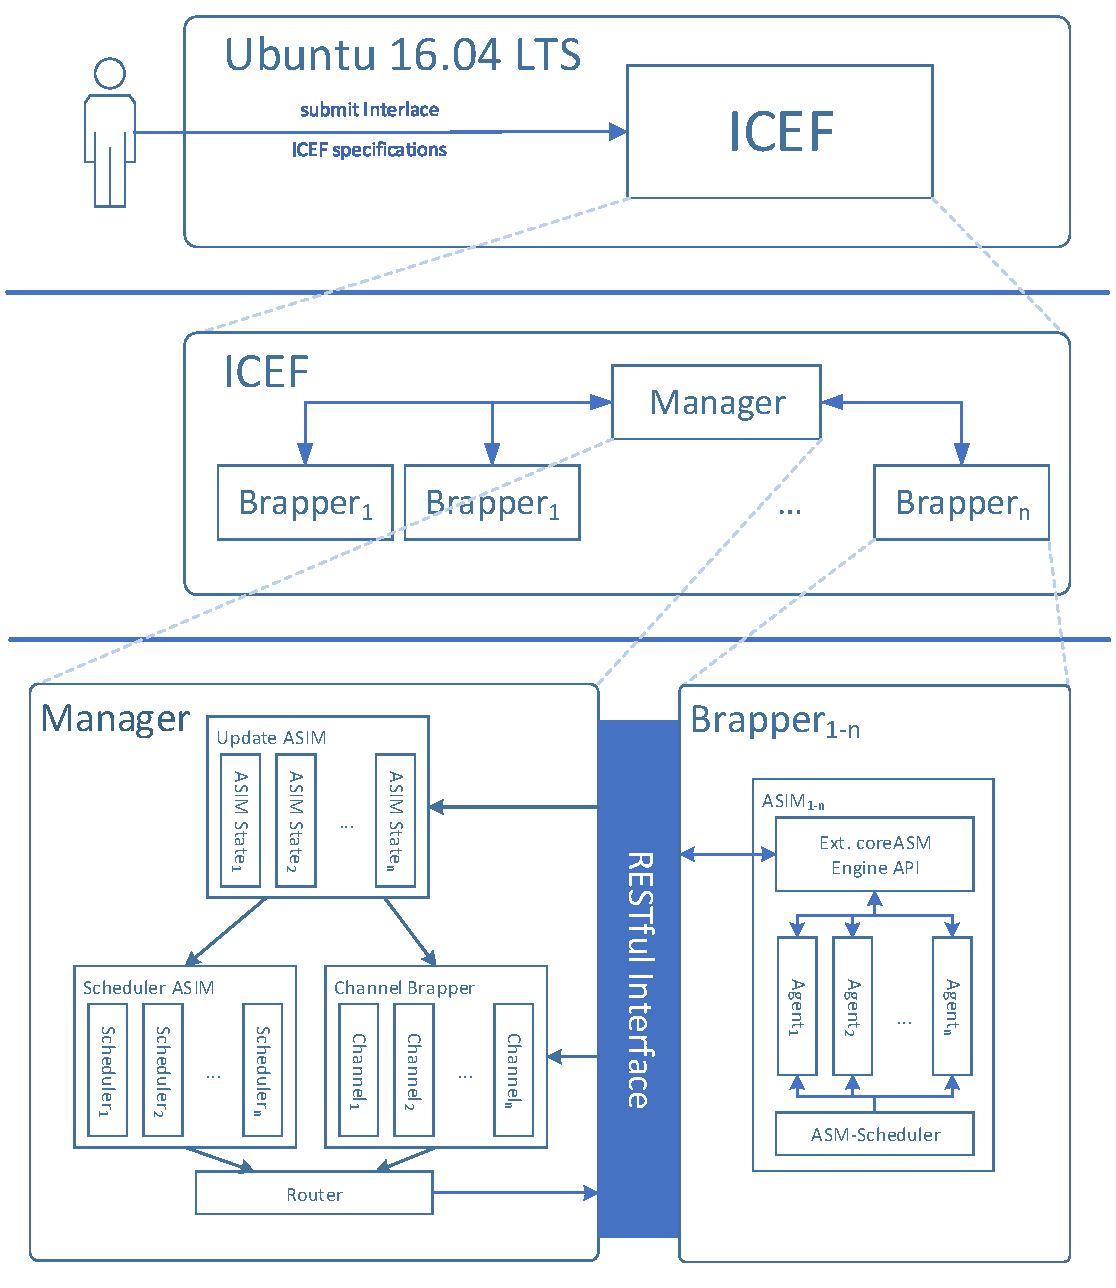
\includegraphics[width=1.0\textwidth, clip, trim=1mm 1mm 1mm 1mm]{Figures/environment_asim}
  \caption{ASIM Execution Environment Overview}
  \label{fig:icef-intro-asim}
\end{figure}

Figure \ref{fig:icef-intro-asim} illustrates on different level of detail which components and services are active and necessary to proved the previously described process running a ASIM simulation and in case of INTERLACE the model specifications.

\subsection{coreASIM}
\label{sec:coreasim-details}

The very core of the Interaction Computer Execution Framework (ICEF) is an engine which has been developed by different people at different universities \footnote{https://github.com/CoreASM/coreasm.core/wiki/About\-CoreASM} and implements a language called ASM. This language is based on Abstract State Machines \cite{BoergerStaerk2003} which is used as a method for high-level system engineering, design and analysis. This engine which is called coreASM got enhanced by the BIOMICS project in order to simulate computer interactions on a logic based programming language.

The resulting engine was called coreASIM including the missing interaction features \cite{BIOMICSD42}\cite{BIOMICSD52} and replaces language ASM by the BIOMICS Specification Language (BSL). The changes from the original framework also comprise of:

\begin{itemize}
	\item interactions possibilities
	\item abstract shared storage
	\item mailing system
	\item full scheduler
	\item interpreter enhancements
\end{itemize}

As this document offers only an overview only the most important implementations are described here, namely the mailbox and the scheduling system. \textbf{The mailing system} can easily be used and can be described as follows:

\begin{minipage}{1.0\textwidth}
An ASIM $asim_1$ can send a message to another ASIM $asim_2$ by using the send message rule.\nopagebreak
\begin{lstlisting}[language=bsl]
	send Element to "asim_2" with subject "a subject"
\end{lstlisting}

Where the \textit{Element} can be of any element location used in ASIM language space. Even for example \textit{programm(self)}.
\end{minipage}

\textbf{The scheduler} has the ability to coordinate different local agents in a way that they act in a predictable and appropriate way. Like the coreASM scheduler coreASIM implements a mechanism controlling at a higher level. At the beginning of each running step, a scheduler takes the defined scheduling policy and is using it to determine a set of local agents which will be signaled to run their program. There are different BSL constructs to do so. Here are two examples:

\begin{lstlisting}[language=bsl]
	forall a in Agents do schedule a
\end{lstlisting}

Which tells the scheduler to run all agents in \textit{Agents}. If a in contrary a single agents should be selected based on a condition $cond$ met by agent $a$, the respective rule might look like this:

\begin{lstlisting}[language=bsl]
	choose a in Agents with cond(a) do schedule a
\end{lstlisting}


\section{Model Execution Environment Details}
\label{sec:exec-env-model-details}



\tikzstyle{every node}=[draw=black,thick,anchor=west]
\tikzstyle{selected}=[draw=red,fill=red!30]
\tikzstyle{optional}=[dashed,fill=gray!50]
\begin{figure}[htbp]
\centering
\begin{tikzpicture}[%
  grow via three points={one child at (0.5,-0.7) and
  two children at (0.5,-0.7) and (0.5,-1.4)},
  edge from parent path={(\tikzparentnode.south) |- (\tikzchildnode.west)}]
  \node {Docker\ Environment}
    child { node {configure}}		
    child { node {Dockerfile}}
    child { node {execute}}
    child { node {README.md}}
    child { node [selected] {scripts}
      child { node {asimrc}}
      child { node {buildICEFDocker.sh}}
      child { node {executeASIMSpec.sh}}
      child { node {runDocker.sh}}
    };
\end{tikzpicture}
\caption{Docker Environment File Structure}
\label{fig:docker-enf-file-struct}
\end{figure}

\todo{scripts, paths, execution}
